% !TEX root = /home/Documents/thesis/draft/thesis.tex
\documentclass[12pt,twoside]{reedthesis}

\usepackage{graphicx,latexsym}
\usepackage{amssymb,amsthm,amsmath}
\usepackage{longtable,booktabs,setspace}
\usepackage{fancyvrb}
\usepackage[hyphens]{url}
\usepackage{rotating}
\usepackage{listings}
\usepackage{fancyvrb}
\usepackage{tikz}
\usepackage[backend=biber, style=numeric, sorting=ynt]{biblatex}
\addbibresource{thesis.bib}

\lstset{	% for source code formatting
basicstyle=\small\ttfamily,
columns=flexible,
breaklines=true
}

\title{A Continued Inquiry into Granularity-Change Cache Simulation}
\author{Alan R. Jessup}
% The month and year that you submit your FINAL draft TO THE LIBRARY (May or December)
\date{May 2024}
\division{Mathematics and Natural Sciences}
\advisor{Charles McGuffey}
\department{Computer Science}

\setlength{\parskip}{0pt}
\begin{document}

\maketitle
\frontmatter % this stuff will be roman-numbered
\pagestyle{empty}

\tableofcontents

% If your abstract is longer than a page, there may be a formatting issue.
\chapter*{Abstract}

...

\mainmatter
\pagestyle{fancyplain}

\chapter{Introduction}

\section{A crash course in computer caching}

Computer memory is the fundamental component of digital systems that serves as a dynamic repository for data and instructions to be temporarily stored for quick access and retrieval during active processes. The drastically lower latency of memory requests compared to retrieval of data from a hard drive or SSD makes memory crucial to efficient performance of computers.

	\subsection*{The memory hierarchy}

	A computer's memory is divided into a \textit{memory hierarchy}, which arranges various types of computer memory in tiers based on side and access speed, with faster but smaller and more expensive layers of memory at the top of the hierarchy. When the processor requests data from memory, each layer of the hierarchy is checked in descending order until the data is located.

	\begin{figure}[h]
    	\centering
    	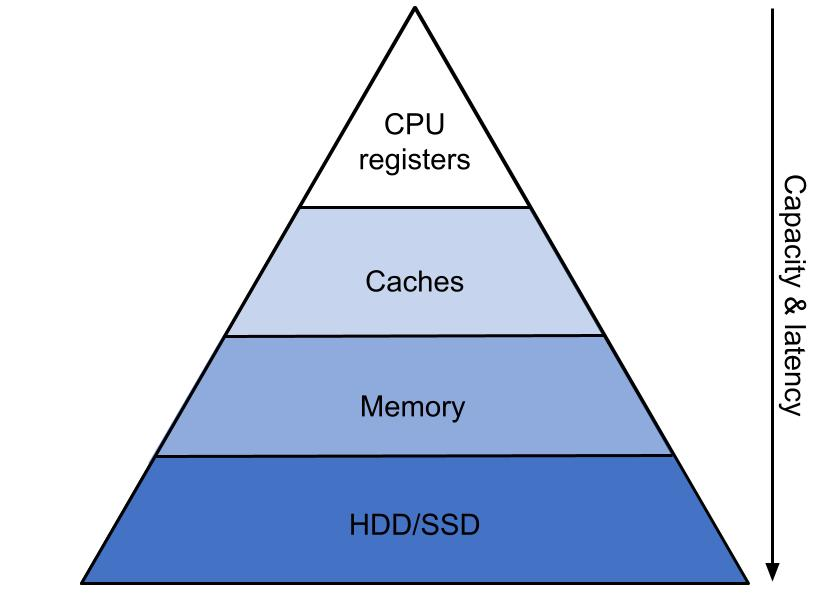
\includegraphics[width=3.5in]{figures/mem_hierarchy.jpg}
    	\caption{A diagram of the memory hierarchy.}
	\end{figure}

	\subsection*{Basics of caching}
	
	The purpose of caching is to reduce the number of accesses made to the main memory by storing data that is highly likely to be requested in the near future. When a piece of requested data is present in a cache, that is called a \textit{cache hit}; when it is absent, it's a \textit{miss}. Since caches are small and fast, intended to be accessed frequently at minimal cost, an important factor of cache design is how to best utilize the limited space they offer to optimize the \textit{hit rate}. The algorithms that caches use to decide which data to store are called \textit{replacement policies}, and are typically designed using \textit{spacial} and \textit{temporal locality}.

	\subsection*{Data locality}

	Locality is a characteristic of data which caches can use to predict what data is likely to be needed next, in order to store that data and reduce latency.
	
	Data with high temporal locality has been used recently; therefore, it is typically more likely to be needed again than any arbitrary other piece of data. Temporal locality is the more common characteristic used in caching, since it can be as simple to implement as a first-in-first-out (FIFO) queue, and is relatively effective on a wide variety of processes.
	
	Data with spacial locality is data that is located in memory physically near other useful data. Caches that make use of spacial locality typically load multiple adjacent lines from memory at the same time. This can be useful in specific cases where a large amount of data is stored sequentially, such as frames of a video. Spatial locality is much less well-studied than temporal locality, which the paper Beckmann et. al. aims to improve through introduction of the \textit{granularity-change caching problem}.

	\subsection*{Caches in realistic systems}

	Although measures of performance such as upper and lower bounds and competitive ratios can be proven for cache models using theoretical analysis and can give a general idea of how a cache model should perform, realistic estimations of cache performance in complex systems require testing to measure outcomes. The introduction of multiprocessing requires \textit{cache coherence protocols} to maintain consistency across shared memory resources, and multiprocessing adds variable of uncertainty into cache performance, since the structure of a specific processor's cache hierarchy or a particular program's implementation of parallelism can complicate cache behavior.

\section{The granularity-change caching problem}

The 2021 paper ``Spatial Locality and Granularity Change in Caching'' describes and provides a theoretical analysis of the Granularity-Change (GC) Caching Problem, which ``modifies the traditional caching setup by grouping data items into blocks, such that a cache can choose any subset of a block to load for the same cost as loading any individual item in the block'' \cite{beckmann}. This allows a cache to take advantage of both spatial and temporal locality, and creates an opportunity to study tradeoffs of cache space usage between the temporally determined \textit{item} cache versus the spatially oriented \textit{block} cache. For the purpose of implementation, Beckmann et. al. describes the deterministic replacement policy \textit{Item-Block Layer Partitioning}.

	\subsection*{Item-Block Layered Partitioning}

	Item-Block Layered Partitioning (IBLP) divides a cache into two virtual segments, one of item granularity and the other of block granularity.

	\begin{figure}[h]
		\centering
		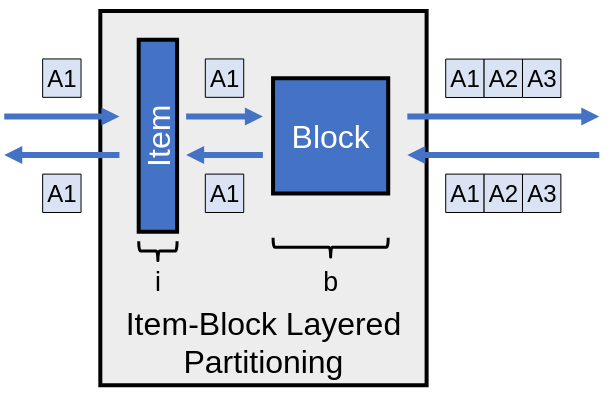
\includegraphics[width=2.5in]{figures/IBLP.png}
		\caption{A diagram of a cache running IBLP \cite{beckmann}.}
	\end{figure}
	
	Beckmann et. al. describes the behavior of IBLP as: \begin{quote}
		The first layer, which serves each access to the cache, loads only the items that are accessed and evicts using the Least-Recently Used (LRU) replacement policy. The second layer, which only serves accesses that miss in the first layer, also uses the LRU policy for evictions, but loads and evicts at the granularity of entire blocks at a time. \cite{beckmann}
	\end{quote}
 
	IBLP models a subset of the granularity-change caching problem for which data is only loaded at the item or block granularity, and never as a subset of a block. This is sufficient for testing the viability of granularity-cache caching, since Beckmann et. al. finds that ``to achieve the best competitive ratio, one should load either an entire block or a single item, and nothing in between'' \cite{beckmann}.
	
	There is no requirement for the relative sizes $i$ and $b$ of the item and block caches in IBLP. Furthermore, Beckmann et. al. determines the optimal layer sizes in IBLP to be unknown, since they depend on the relative spatial and temporal locality of a particular trace, and recommends further analysis. This makes relative layer sizes a useful variable for furthering understanding of granularity-change caching.


\section{Prior work simulating GC caching}

In 2022, the Reed College thesis titled ``Simulating the Granularity-Change Caching Problem'', by Maxx Curtis, follows-up the theoretical work of Beckmann et. al. on the granularity-change caching problem by providing a foray into practical simulation of the proposed cache model. Curtis provides a survey of two systems simulators, Zsim and Gem5, and a presents a custom implementation of a block Cache in Gem5 \cite{curtis}.

	\subsection*{Block cache implementation}

	The block cache implemented by Curtis is built from the ground up as a new object, and thus is limited in what features of a Gem5 system it can be configured with. It operates on the level of handling packet streams between the CPU/caches, and facilitates the switch between item and block granularity at this level. 

	The ``Shortcomings'' section of Curtis explains that due to the time-consuming nature of this low-level implementation, the block cache is only usable in simple systems with a single cache level and ``Simple Timing CPU'', a ``unrealistic but very fast CPU model'' \cite{curtis}. Therefore, one of the priorities of my work here is to provide an implementation that allows for use in more realistic system configurations.

	Unfortunately the code from the Curtis thesis was unavailable, so continuing to build on this implementation of the block cache was not a possibility.

	\subsection*{Results of Curtis}

	Curtis tests three cache configurations against each other: a simple one-level cache of item granularity, a simple one-level cache using the custom block cache, and an IBLP cache constructed using a standard cache of item granularity in conjunction with a block cache. Three benchmarks are used: iterative merge sort (high in spacial locality), randomized subset-sum (high in temporal locality), and recursive merge sort (a combination of both forms of locality).
	
	\begin{figure}[h]
		\centering
		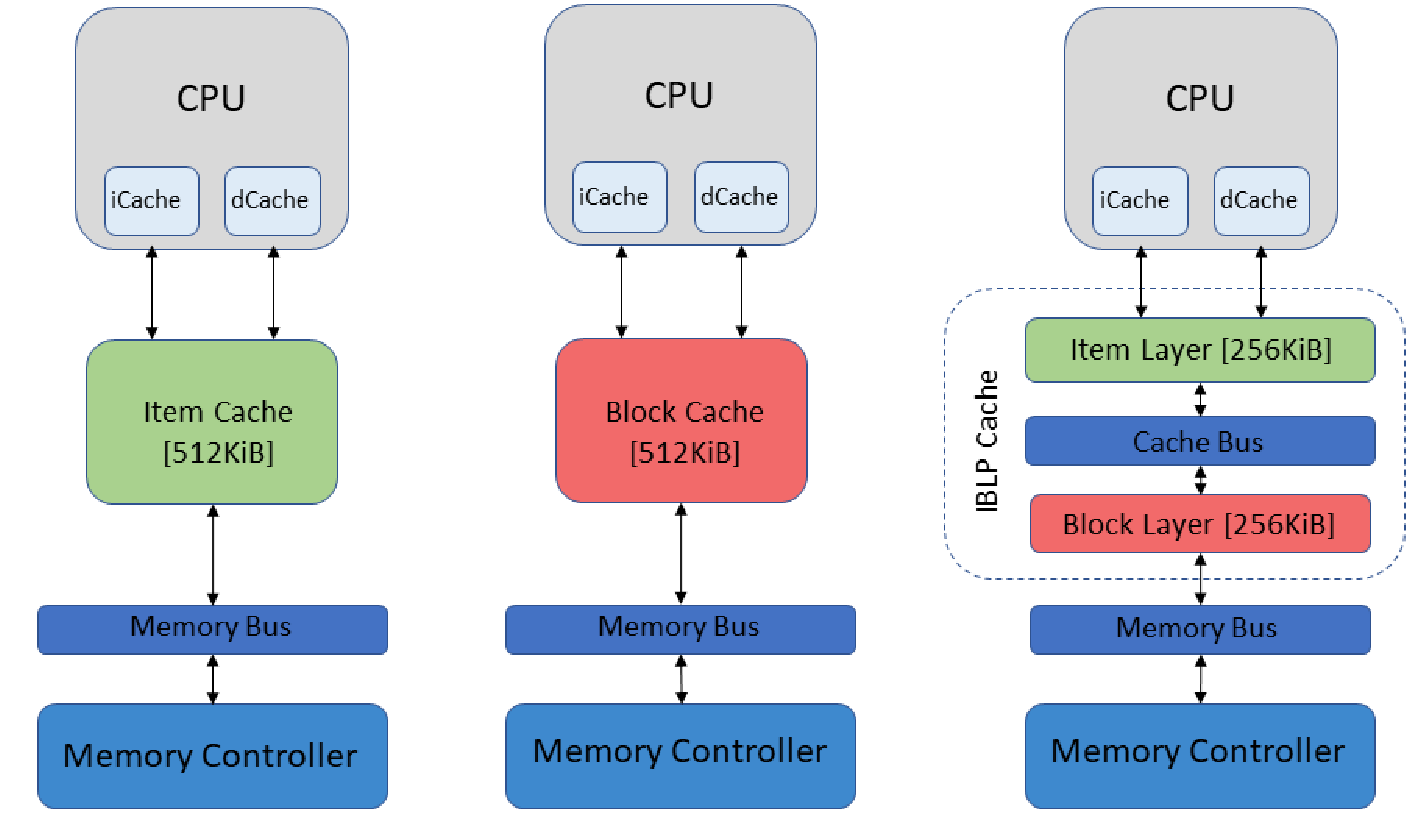
\includegraphics[width=5in]{figures/curtis_caches.png}
		\caption{The three cache configurations tested by Curtis \cite{curtis}.}
	\end{figure}

	Both merge sort scripts result in a a hit rate near $100\%$ for all three cache types, and randomized subset-sum results in a hit rate near $99.5\%$ for the item and block caches and near $95.5\%$ for the IBLP cache \cite{curtis}. Since this does not line up with the expectation of poor performance of the item cache for high spacial locality and poor performance of the block cache for high temporal locality, the results of these tests are inconclusive.

	\begin{figure}[h]
		\centering
		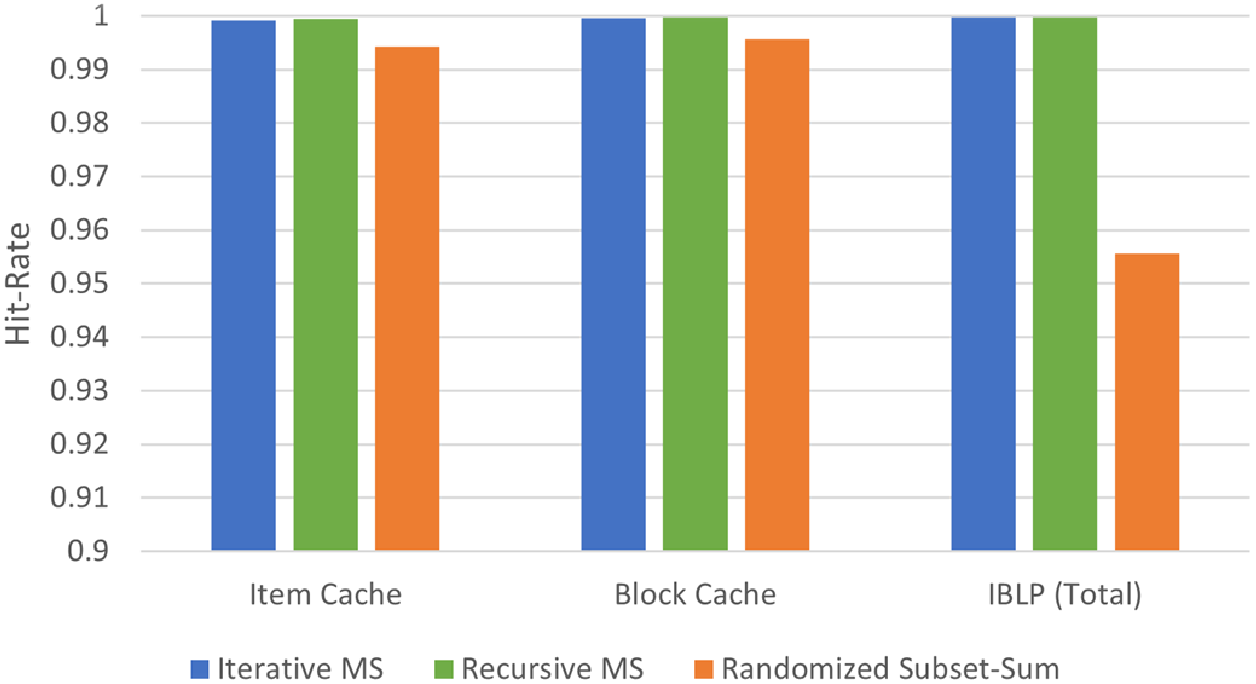
\includegraphics[width=4.8in]{figures/curtis_cache_hit_rates.png}
		\caption{Hit rates resulting from tests of the three cache configurations \cite{curtis}.}
	\end{figure}

	Furthermore, looking specifically at the hit rates of the individual layers of the IBLP cache, the three test scripts do not support the expectation of a positive corelation between high spacial locality and high relative utilization of the block layer.

	\begin{figure}[h]
		\centering
		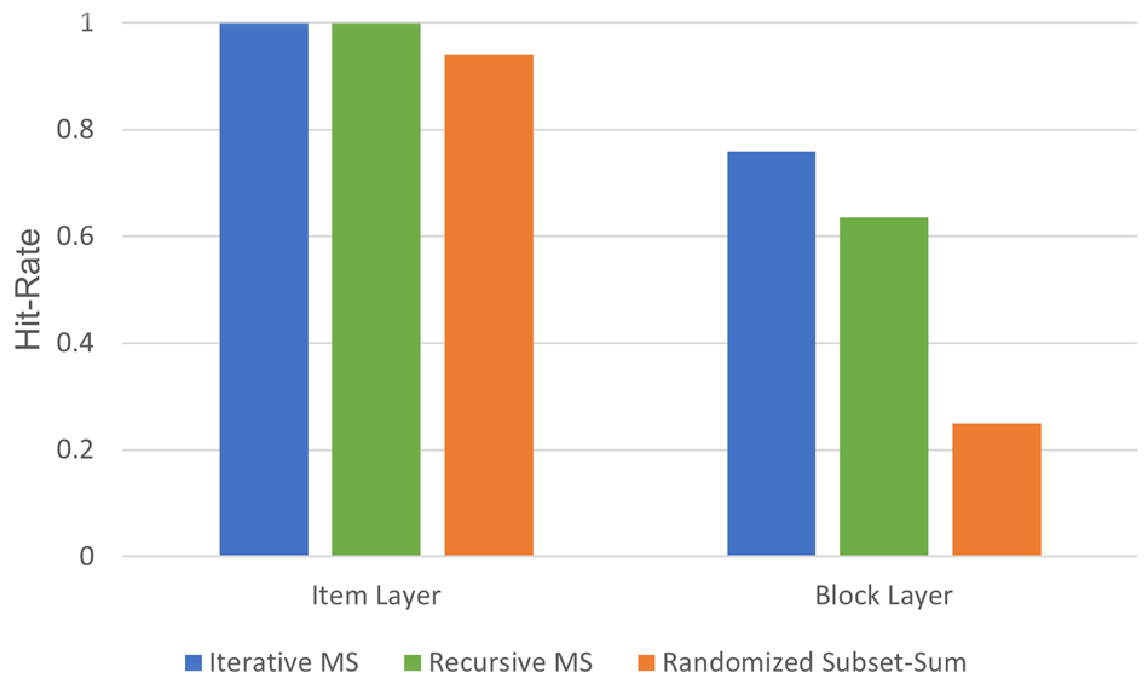
\includegraphics[width=4.5in]{figures/curtis_layer_hit_rates.png}
		\caption{Hit rates for the item and block layers of the IBLP cache \cite{curtis}.}
	\end{figure}

	Curtis suggests that these inconclusive results are due in part to the high granularity of the block layer in the IBLP cache, and insufficient memory workload of the test scripts compared to the caches' sizes. These factors are thus important to keep in mind when designing future tests to measure performance of granularity-change caches.

	\subsection*{Suggestions for future work}

	In conclusion, Curtis states: \begin{quote}
		At this stage of development, I recommend against using my implementation for further research into IBLP. ... If one only wanted to examine the viability of IBLP itself, then it would be fairly easy to use typical Cache objects to do so... by creating a system with two caches, one for each layer, that differ in granularity and experience little to no intermediate latency. \cite{curtis}
	\end{quote}

	Additionally, Curtis suggests working towards an implementation of a granularity-change cache model that is compatible with more realistic processors than Gem5's simple CPU models. Since Gem5 has a wide variety of available CPU models, this is a matter of compatibility with the full array of cache features in Gem5, including response queues and cache coherence.


\section{Approach}

With the results and suggestions of the Curtis thesis in mind, my approach to further research on the granularity-change caching problem is to build and test a modular implementation of IBLP using the existing Gem5 cache objects. Since the existing Gem5 caches are compatible with the full range of Gem5's features, an implementation using these caches as its foundation should be able to maintain these compatibilities, thereby eliminating the need for laborious re-implementation of Gem5's cache features from the ground up.


%%%%%%%%%%%%%%%%%%%%%%%%%%%%%%%%%%%%%%%%%%%%%%%%%%%%%%%%%%%%%%%%%
\chapter{Attempting a modular IBLP implementation in Gem5}

\section{Overview of Gem5}

Gem5 is an open-source, community-led computer computer systems simulation project that describes itself as: \begin{quote}
	...a modular platform for computer-system architecture research, encompassing system-level architecture as well as processor microarchitecture. \cite{gem5-about}
\end{quote}

Gem5 began as two separate projects, m5 at the University of Michigan and GEMS at the University of Wisconsin, until the two simulators were merged in 2011 \cite{gem5-about}.

	\subsection*{Caching subsystems}

	Due to its origins as a combination of m5 and GEMS, Gem5 contains two separate subsystems that can both be used to model caches. The \textit{classic} cache model from m5 provides simple, modular functionality for multi-level caches, but with an inflexible MOESI cache coherence protocol. The \textit{Ruby} cache model has more complex implementation details, with the ability to test customized cache coherence protocols.

\section{Initial classic cache implementation}

	I began by implementing a nestled cache structure using classic Gem5 caches. This involved first building a simple cache configuration following the Gem5 documentation's ``Getting Started'' tutorial, then modifying the cache bus configuration to support a nestled block layer and writing a wrapper program to perform trials and collect data from the simulation.

	\subsection*{Config files}

	A Gem5 configuration is defined by a python file in the ``configs'' directory. To run a config, the path to this file is given to the appropriate build command for the config's architecture, along with any arguments such as the path of the script to simulate.
	
	Contained within a config file are the commands to create a system object, set up a system, and start a simulation.

	\subsection*{System class}

	For the purpose of organizing and modularizing the facets of the Gem5 system configuration that are peripheral to the IBLP implementation, such as processor initialization and simulation execution, I implemented the system setup in a new class, \verb`StreamlinedSystem`. This class inherits the Gem5 \verb`System` class and adds the following methods to take care of setting up the components of a typical system for simulation and piecing together the components of the IBLP cache:

	\begin{itemize}
		\item \verb`__init__(self)` sets up the system attributes that are needed for setting up other features: clock, voltage, memory mode and ranges, cpu, and busses for between L1 and L2 caches.
	
		\item \verb`setup_caches(self, cache_type)` sets up and connects busses to the caches: the L1 instruction and data caches, which have constant configurations, and the L2 cache, which is configured as either an Item, Block, or IBLP cache.
	
		\item \verb`setup_memory(self)` sets up the main memory and connects it to the L2 cache bus.
	
		\item \verb`run(self, binary)` sets the simulation up to run as a process, and runs it.
	\end{itemize}

	The specific commands for of most of these steps, except for \verb`setup_caches`, are adapted from the gem5 tutorial \cite{gem5-tutorial}.

	\subsection*{Cache objects}

	A basic classic cache configuration requires minor setup of cache objects and busses; this encompasses L1 data and instruction caches, which are specialized caches with ports specified in the System object, and a general L2 cache which I adapted into a nestled item and block cache:

	\begin{itemize}
		\item \verb`L1Cache`, \verb`DataCache`, and \verb`InstructionCache` are adapted from the gem5 basic caches tutorial to mimic the typical on-processor data and instruction caches in an ordinary system.
	
		\item \verb`L2Cache` contains the attributes of a typical L2 cache that are shared by both item and block caches.
	
		\item \verb`ItemCache` and \verb`BlockCache` inherit from \verb`L2Cache` and set up the structure for the two-part IBLP cache.
	
		\item \verb`IBLPCache(ItemCache)` simulates an IBLP cache by using an item cache, connected on the memory-side to a block cache, with attributes set so that there is minimal latency between these two caches. The method \verb`connectMemSideBus` is altered to connect the block layer to the memory bus, to imitate the way the memory connects to layers in the IBLP cache model.
	\end{itemize}

	\subsection*{Variable parameters}

	Since there are a number of parameters of the cache objects that should be adjusted and fine-tuned during testing, I created \verb`options.json` to be read by the file where the cache objects are defined, and used to set cache attributes accordingly.

	\subsection*{Wrapper script}

	The wrapper file \verb`main.py` runs Gem5 with the config and measures the output written to \verb`stats.txt` at the end of each simulation. It's necessary that statistics be collected using a file outside the config because gem5 doesn't write to `stats.txt` until the simulation has terminated, and doesn't make these available during the running of a simulation.

	The wrapper takes the three arguments to customize trials: the path to the binary of the script to simulate, the cache models to be tested (out of Block, Item, and IBLP), and the number of trials to run of each cache type.

\section{Granularity limitations}

	The crucial limitation of my initial classic cache implementation is that it relies on Gem5 having a way, such as through a cache object attribute, to specify the line size for any given layer of memory.

	Instead, Gem5 sets an attribute for line size at the level of the \verb`System` class. This prevents any possibly implementation of granularity-change caches in classic caches without modification of Gem5's \verb`System` and \verb`Cache` classes to allow specification of a larger line size for memory.


\section{Considering Ruby for granularity change}

	Since my initial classic cache implementation failed to meet the requirements for simulating an IBLP cache, I turned to the Ruby cache system to see if the more detailed cache model includes a way of overriding the system-wide line size requirement.

	\subsection*{Overview of Ruby}

	Ruby provides a detailed system for simulating memory systems with a wide array of configurations, including ``inclusive/exclusive cache hierarchies with various replacement policies, coherence protocol implementations, interconnection networks, DMA and memory controllers'', and more \cite{gem5-ruby}.

	\begin{figure}[h]
		\centering
		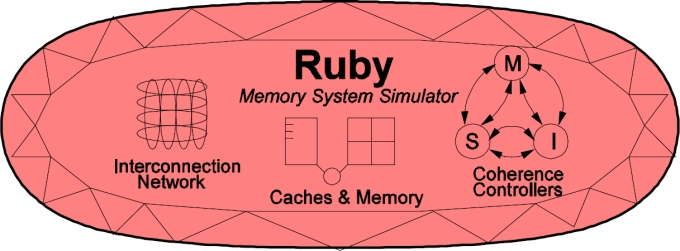
\includegraphics[width=4.5in]{figures/ruby.jpg}
		\caption{A graphic from GEMS visualizing Ruby's components \cite{gem5-ruby}.}
	\end{figure}

	For my purpose, a simple but realistic memory system is sufficient to model IBLP, so most of the features of a Ruby cache system are unnecessary. However, implementation of a granularity-change-capable cache in Ruby would provide countless options for future research studying the intersection of granularity-change in caches with other complicating variables.

	\subsection*{Cache coherence specification}

	Ruby specifies cache coherence protocols using ``Specification Language for Implementing Cache Coherence'' (SLICC). These files are written in the ``src'' directory, and have to be compiled with a new build of Gem5, unlike configs. They do not provide any interaction with memory allocation that would allow for manipulation of cache granularity.

	\subsection*{Ruby architecture}

	Unlike classic caches, where cache objects are each individually connected with the system, Ruby cache objects are defined as cache controllers within a network and configured within a cache system.
	
	In the example from ``Learning Gem5'', the cache system named \verb`MyCacheSystem` is configured with a \verb`L1Cache` that inherits \verb`L1Cache_Controller`, a \verb`DirController` that inherits \verb`Directory_Controller`, and a memory network \verb`MyNetwork` inheriting \verb`SimpleNetwork` \cite{gem5-tutorial}.

	Since the matter of implementing granularity-change caching only concerns the architecture within a particular cache, only the \verb`L1Cache` is of significance. The \verb`L1Cache` object is defined with the following methods: \begin{itemize}
		\item \verb`versionCount` and \verb`getBlockSizeBits` are simple helpers for \verb`__init__`
		\item \verb`__init__` initializes the memory controller by defining its memory and connecting it to the system components
		\item \verb`sendEvicts` and \verb`connectQueues` manage components of cache coherence
	\end{itemize}

	Within \verb`__init__`, the memory definition provides the only config-level mention of block size: \begin{verbatim}
self.cacheMemory = RubyCache(
    size="16kB", assoc=8, start_index_bit=self.getBlockSizeBits(system)
)\end{verbatim}

	The helper \verb`getBlockSizeBits` here is a simple conversion of the system-level line size value, and thus can't be manipulated to modify the line size since it only determines the start bit offset. There is no evidence that Ruby offers any opportunities to manipulate individual-cache line size not present in a classic cache.

	\subsection*{Limitations}

	Since the Ruby caches, like the classic caches, operate under the assumption of a constant system-wide line size, there is no evident way to modify the granularity of individual memory layers using Ruby without extensive modification, to the degree of the Curtis block cache implementation or greater.

	Furthermore, the complexity of the Ruby subsystem is such that it would not be advisable to implement IBLP in Ruby unless specifically for the purpose of studying granularity-change caching in conjunction with features specific to Ruby, such as cache coherence.

\section{A closer look at system-scope granularity}

	The final possibility of implementing IBLP using existing Gem5 cache objects would be if relatively small modifications could be made to the Gem5 source code to change the granularity parameter, where it receives the system-assigned line size, to instead use a custom line size value.

	\subsection*{Cache interface source code}

	I began by inspecting the Python interface for the classic cache base object, defined in \verb`gem5/src/mem/cache/Cache.py`. This file contains python interfaces for the following C++ classes:
	\begin{itemize}
		\item \verb`Clusivity`, an enum type object used to specify the behavior of a cache in regard to upstream caches as ``mostly inclusive'' or ``mostly exclusive''.
		\item \verb`WriteAllocator`, which is used for allocating memory for cache writes and invokes \verb`Parent.cache_line_size` to set its own \verb`block_size` attribute.
		\item \verb`BaseCache`, the parent class from which other cache objects inherit basic functionality.
		\item \verb`Cache`, the object used to create L1 and L2 caches in a config.
		\item \verb`NoncoherentCache`, to use as a last-level cache in multiprocessor systems.
	\end{itemize}

	At the interface level alone, the most that could be done to alter granularity of a specific cache is to overwrite \verb`WriteAllocator.block_size` with a new parameter, either passed down through the `Cache` constructor or through the system object as \verb`Parent` the same way that \verb`cache_line_size` is passed. This alteration would be required in conjunction with modification of all relevant C++ class definitions.

	\subsection*{Cache class definition source code}

	The C++ source code for the \verb`Cache` object, found in \verb`gem5/src/mem/cache/cache.cc`, contains definitions for 22 methods, many of which invoke inherited \verb`BaseCache` methods. These methods handle the actual passing of packets in and out of caches, including details of timing, eviction behavior, and snooping.

	The only reference to the system-level line size is where the \verb`Cache` constructor passes it to its parent `BaseCache`, on line 70 with:
	\begin{verbatim}
Cache::Cache(const CacheParams &p)
    : BaseCache(p, p.system->cacheLineSize()),
      doFastWrites(true)
	\end{verbatim}
	This parameter of \verb`BaseCache` is then used to set the attribute \verb`blkSize`. It would thus be simple to overwrite the value of \verb`blkSize` with a cache-specific custom granularity by replacing this use of \verb`p.system->cacheLineSize()` with either a custom system attribute or new constructor parameter.

	The use of block size following this appears well-contained to the scope of the \verb`Cache` class, only being used through the attribute \verb`blkSize`, which is referenced 15 times in \verb`cache.cc`. It is frequently used in conjunction with the \verb`Packet` method `getSize()`, and is only used in the context of packet operations.
	
	A cursory inspection of \verb`gem5/src/mem/cache/base.cc`, which contains the definitions for both \verb`BaseCache` and \verb`WriteAllocator`, shows similar usage and no references to the system-level line size via \verb`p.system->cacheLineSize()`. The base cache does have access to \verb`system` and its attributes, but only uses this in the context of handling requestors.
	
	From a cursory inspection of the \verb`Packet` source code in \verb`gem5/src/mem/packet.cc`, the \verb`Packet` class appears to be well-contained as well, with no evidence to suggest it would interfere with modification of higher-level objects.

	\subsection*{Complicating factors}

	There are a few points of complication to attempting to modify Gem5's cache object source code, namely the implementation details of translating packet granularity, and the potential for errors caused by widespread access to system-level attributes.
	
	Since Gem5 is not built to accommodate translating memory packets between granularity, setting a different line size between cache layers will result in fatal errors unless packets are transformed between layers. This could potentially be solved with a custom cache bus, but only if the Gem5 source code is sufficiently modular that the modification of line size at the memory level would not interfere with line size at the processor level.
	
	Gem5 does have excellent modularity at the configuration level, as far as the ability to mix-and-match components, but modification of these components' source code in regard to system-level attributes is complicated by the fact that most low-level objects inherit access to system-level attributes. This makes it challenging to isolate objects from attributes of the \verb`System` instance, and makes it unlikely that the line size of an individual cache could be modified without identifying and accounting for all reference to the \verb`System` object's line size at lower levels.

	A cursory search using \verb`grep -r "p.system->cacheLineSize"` in \verb`gem5/src` shows only 11 references to \verb`p.system->cacheLineSize`, so replacing each of these instances could be doable. However, given the likelihood of unforeseen impacts on peripheral components, in practice this would likely be a much more daunting task to implement and troubleshoot.

	\subsection*{Conclusion on granularity-change implementation in Gem5}

	Given the significant complication of modifying the source code of Gem5 caches to implement a granularity-change functionality and the lack of evidence of any simpler method of implementing granularity-change caching in Gem5, I have concluded that further work implementing IBLP in Gem5 in its current state is not a worthwhile pursuit.

	I will instead present a study of alternative options for cache simulation with a focus on their capacity for mixed granularity cache implementation.

%%%%%%%%%%%%%%%%%%%%%%%%%%%%%%%%%%%%%%%%%%%%%%%%%%%%%%%%%%%%%%%%%

\chapter{Next section}

\section{Something or other}

%%%%%%%%%%%%%%%%%%%%%%%%%%%%%%%%%%%%%%%%%%%%%%%%%%%%%%%%%%%%%%%%%
\chapter{Conclusion}

\section{Results}

...

\section{Future work}

...

%%%%%%%%%%%%%%%%%%%%%%%%%%%%%%%%%%%%%%%%%%%%%%%%%%%%%%%%%%%%%%%%%
\appendix
\chapter{Glossary}

\def\arraystretch{1.5}
\begin{tabular}{p{1.5in}p{3.8in}}
    \hline
    \textbf{Term}       & \textbf{Definition} \\
    \hline
	Associativity		& ... \\
	Block               & In the context of general caching, a standard amount of data. \\
	Block (GC-cache)	& In granularity-change caching, \textit{block} specifically refers to the lower-granularity line size. \\
	Cache coherence		& ... \\
	Granularity         & The size of a data \textit{block}, i.e. cache \textit{line}. A higher granularity has a larger block size, and lower vice versa. \\
	Competitive ratio	& ... \\
	Hit/miss rate 		& ... \\
    Item (GC-cache)  	& In GC-caching, \textit{item} refers to the higher-granularity line size. \\
    Line                & A portion of a cache that contains one \textit{block} of data. \\
	Memory hierarchy	& ... \\
\end{tabular}

%%%%%%%%%%%%%%%%%%%%%%%%%%%%%%%%%%%%%%%%%%%%%%%%%%%%%%%%%%%%%%%%%
\chapter{Source code and documentation}

\section{Simulation config}

\subsection*{Caches}
%\lstinputlisting{code/msi_caches.py}
\;\\

\subsection*{Runfile (Config)}
%\lstinputlisting{code/simple_ruby.py}
\;\\

\section{Test scripts}

...

\backmatter % backmatter makes the index and bibliography appear properly in the t.o.c...

\nocite{*}
\addcontentsline{toc}{chapter}{References}
\printbibliography[title=References]

\end{document}
